\section{Magnesium chloride solutions in DME}

In this section, spectral data obtained from AIMD simulations for systems marked as III and IIIa-c in section~\ref{section:mg-cl-dme-structural} are described. It was published in the article~\cite{mg-cl-dme}.

\begin{figure}[ht]
    \centering
    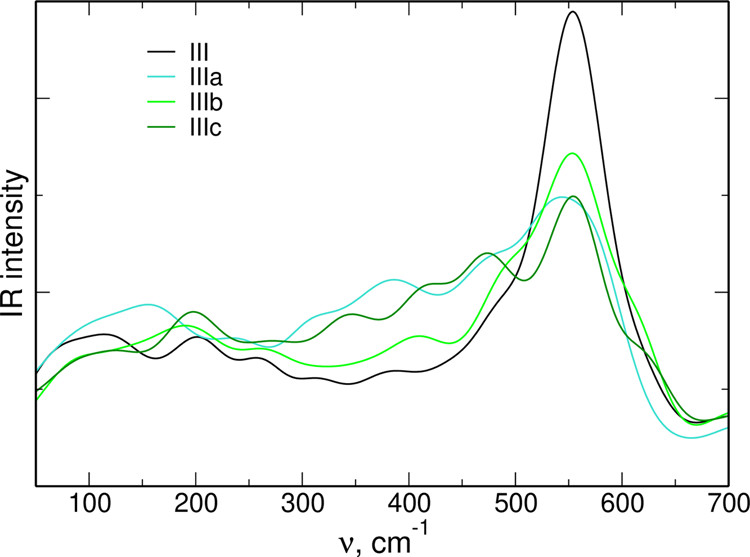
\includegraphics[width=0.4\textwidth]{img/4-ir-spectra-from-aimd-simulations/2-mg-cl-dme/ir-aimd.png}
    \caption{IR spectra obtained from AIMD trajectories for systems III and IIIa-c}
    \label{fig:mg-cl-dme-ir-aimd}
\end{figure}

Figure~\ref{fig:mg-cl-dme-ir-aimd} shows IR spectra obtained from AIMD trajectories. For systems with initially aggregated ions (IIIa-c) there is an increase in intensity in the range 300-450~cm$^{-1}$ with respect to system~III. Based on the results of vibrational analysis from QC calculations~\cite{mg-cl-dme} (not described here), it can be attributed to Mg$_2$Cl$_2^{2+}$ and Mg$_3$Cl$_4^{2+}$ aggregates. Additionally, the band at about 550~cm$^{-1}$ may be assigned to TFSI$^{-}$ anions.

\begin{figure}[ht]
    \centering
    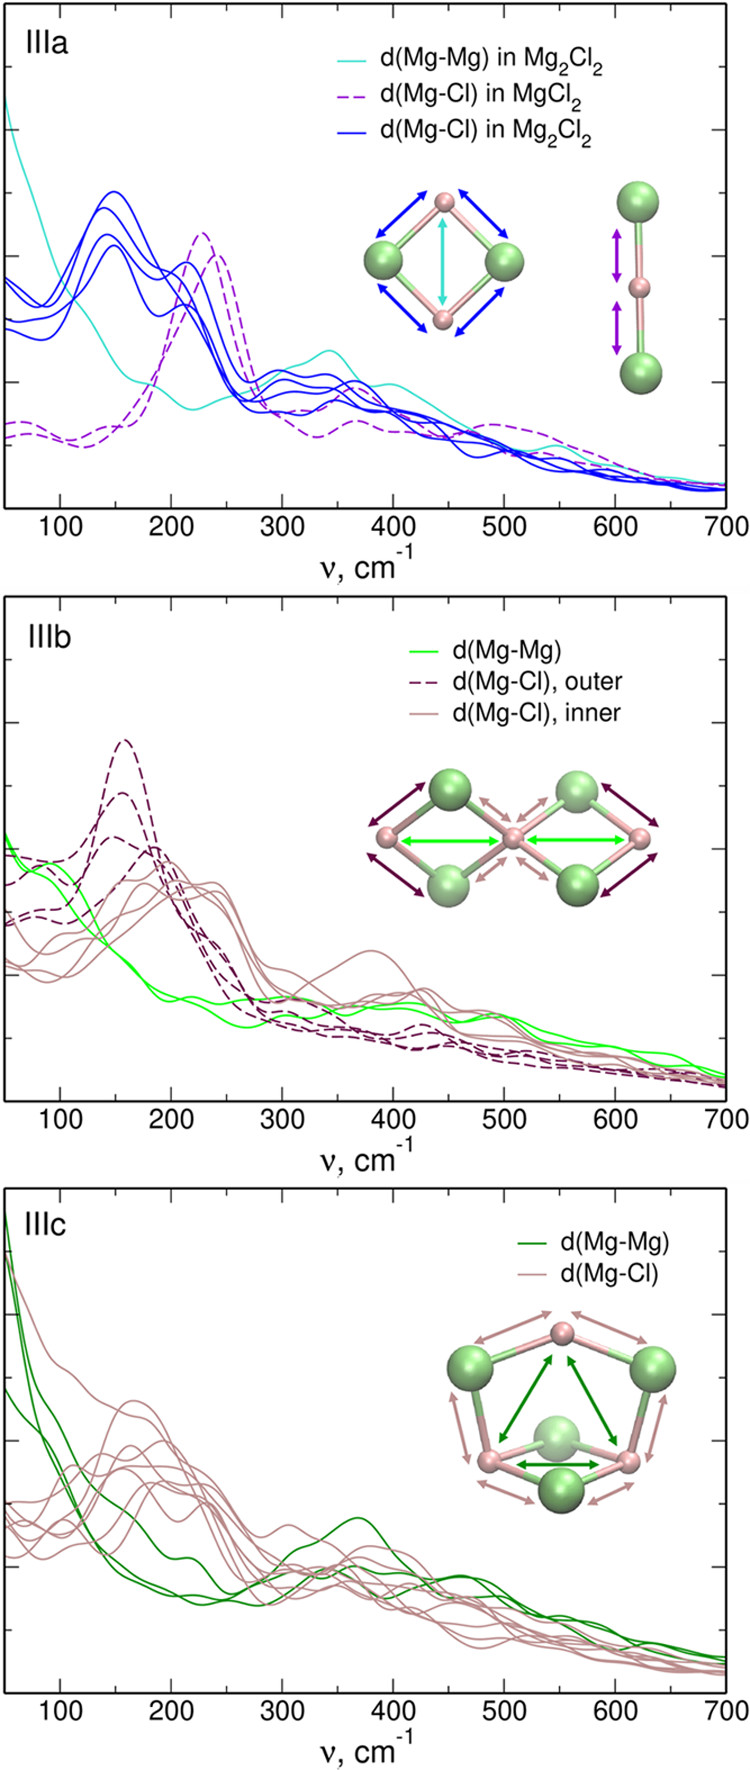
\includegraphics[width=0.4\textwidth]{img/4-ir-spectra-from-aimd-simulations/2-mg-cl-dme/ft-mg-mg.png}
    \caption{Fourier transforms of Mg-Mg and Mg-Cl distances obtained from AIMD simulations for systems IIIa-IIIc}
    \label{fig:mg-cl-dme-ft-mg-mg}
\end{figure}

As for the NaFSI/EMIM-FSI systems, FTs of individual structural parameters were calculated. Selected results are presented in Figure~\ref{fig:mg-cl-dme-ft-mg-mg}. For Mg-Mg distances observed modes have frequencies below 100~cm$^{-1}$ but for IIIa and IIIc there are also contributions at about 350~cm$^{-1}$. Therefore, the observed increase in intensity in IR spectrum may be related to these displacements. For all systems containing aggregated ions in the initial structures (IIIa, IIIb and IIIc), the vibrations of Mg-Cl distances appear between 150 and 250 cm$^{-1}$. Comparison of these plots shows the difference between frequencies of Mg-Cl vibrations in different environments: the frequencies for MgCl$_2$ in IIIa are higher than for Mg$_2$Cl$_2^{2+}$. Similarly in IIIb system, for the linear complex Mg$_3$Cl$_4^{2+}$, frequencies of Mg-Cl stretching vibrations are different for inner and outer Mg$^{2+}$ ions.

\begin{figure}[ht]
    \centering
    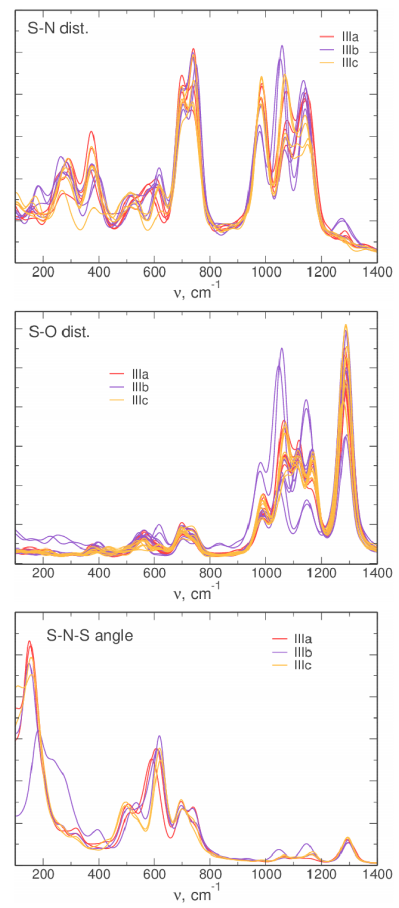
\includegraphics[width=0.4\textwidth]{img/4-ir-spectra-from-aimd-simulations/2-mg-cl-dme/ft-s-o-angles.png}
    \caption{Fourier transforms of geometric parameters of TFSI$^{-}$ anions from the AIMD simulations}
    \label{fig:mg-cl-dme-ft-s-o-angles}
\end{figure}

To prove the assignment of the 550~cm$^{-1}$ band to TFSI$^{-}$ anion, FTs of S-O and S-N distances and the S-N-S angles were calculated and are shown in Figure~\ref{fig:mg-cl-dme-ft-s-o-angles}. From plots for S-N bonds and S-N-S angles it is clear that the modes at 550-600~cm$^{-1}$ are related to these vibrations in every system. For the S-O stretching in system IIIb a~pattern differing from the other systems is observed in the range 1000-1200~cm$^{-1}$. In addition, in this case there are large differences between individual bonds within the same system.

\begin{figure}[ht]
    \centering
    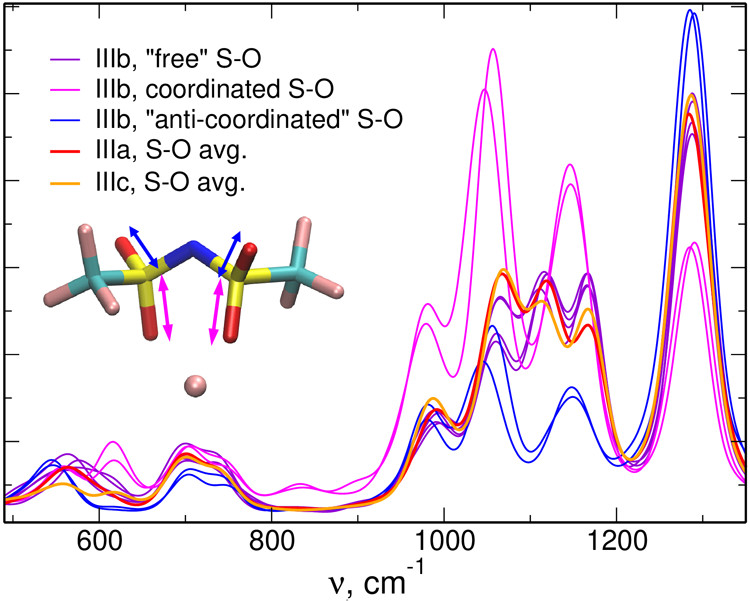
\includegraphics[width=0.4\textwidth]{img/4-ir-spectra-from-aimd-simulations/2-mg-cl-dme/ft-s-o.png}
    \caption{Fourier transforms of S-O bond lengths in TFSI$^{-}$ anions, for systems IIIa and IIIc the averages over all bonds are presented while for system IIIb FTs for individual bonds are shown}
    \label{fig:mg-cl-dme-ft-s-o}
\end{figure}

In Figure~\ref{fig:mg-cl-dme-ft-s-o} plots of FTs for S-O distances are presented. In each of systems IIIa-c, there were 8~S-O bonds in TFSI$^{-}$ anions. It was observed that for systems IIIa and IIIc FTs of all of them are similar, so only averages over all S-O bonds for these systems are presented. It is no longer the case for IIIb system in which from eight S-O bonds, FTs for four of them are similar to those for systems IIIa and IIIc, whereas two S-O pairs are different. This effect is related to the fact, that IIIb system is the only one containing one TFSI$^{-}$ anion coordinated to Mg$^{2+}$ cation. Two different pairs of S-O bonds are the bonds either coordinated to Mg$^{2+}$ cation or pointing in the opposite direction. For these bonds, positions of maxima of FT differ from those observed for "free" S-O bonds (in IIIa and IIIc systems and for four other S-O bonds in system IIIb). So, in this way it is possible to discern vibrational frequencies of "free" bonds and bonds involved in coordination during analysis of vibrational spectra of the system.

As it has been seen in Figure~\ref{fig:mg-cl-dme-ft-mg-mg} and also from QC data in~\cite{mg-cl-dme}, different Mg$_x$Cl$_y^{(2x - y)}$ aggregates are involved in vibrations with similar frequencies, thus to differentiate them, study of changes appearing in the IR spectrum with changing composition of electrolyte (solvent, concentrations, Mg:Cl ratio) is needed.

\cleardoublepage